\chapter*[Arquitetura]{Arquitetura}
\addcontentsline{toc}{chapter}{Arquitetura}

\section{Visão Geral}

\begin{figure}[!h]
    \centering
    \caption{Visão Geral - Parte 1}
    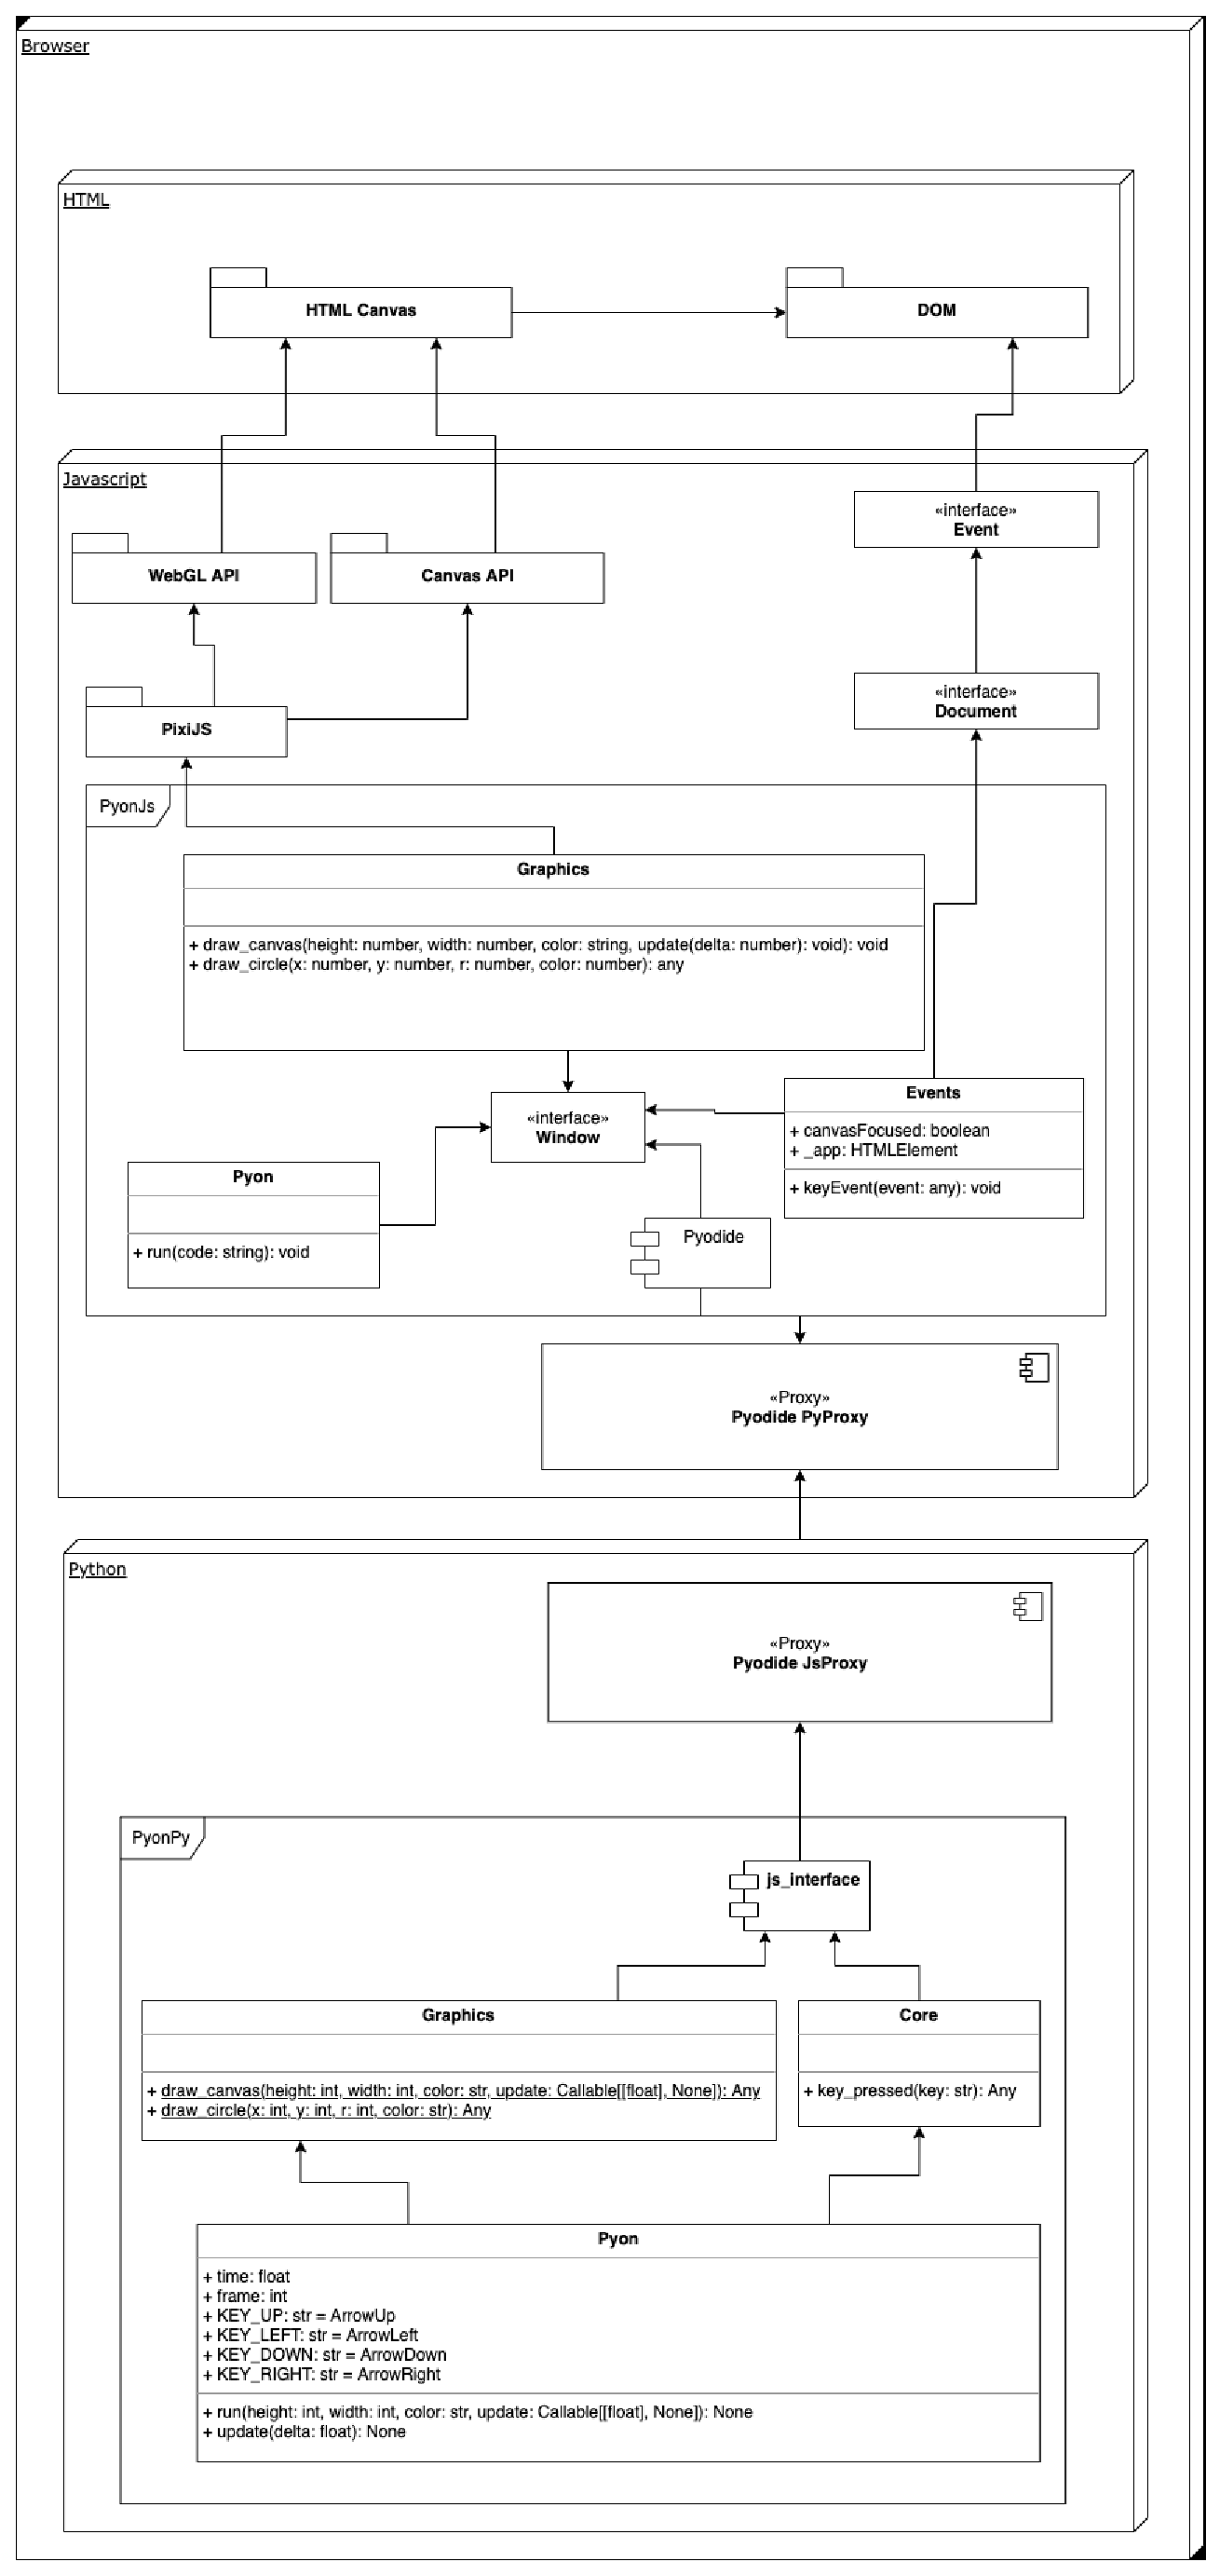
\includegraphics[trim={0 23cm 0 0},clip,keepaspectratio=true,scale=0.8]{figuras/Arquitetura.eps}
    \legend{Fonte: Autores}
    \label{fig:arquitetura}
\end{figure}

\begin{figure}[!h]
    \centering
    \caption{Visão Geral - Parte 2}
    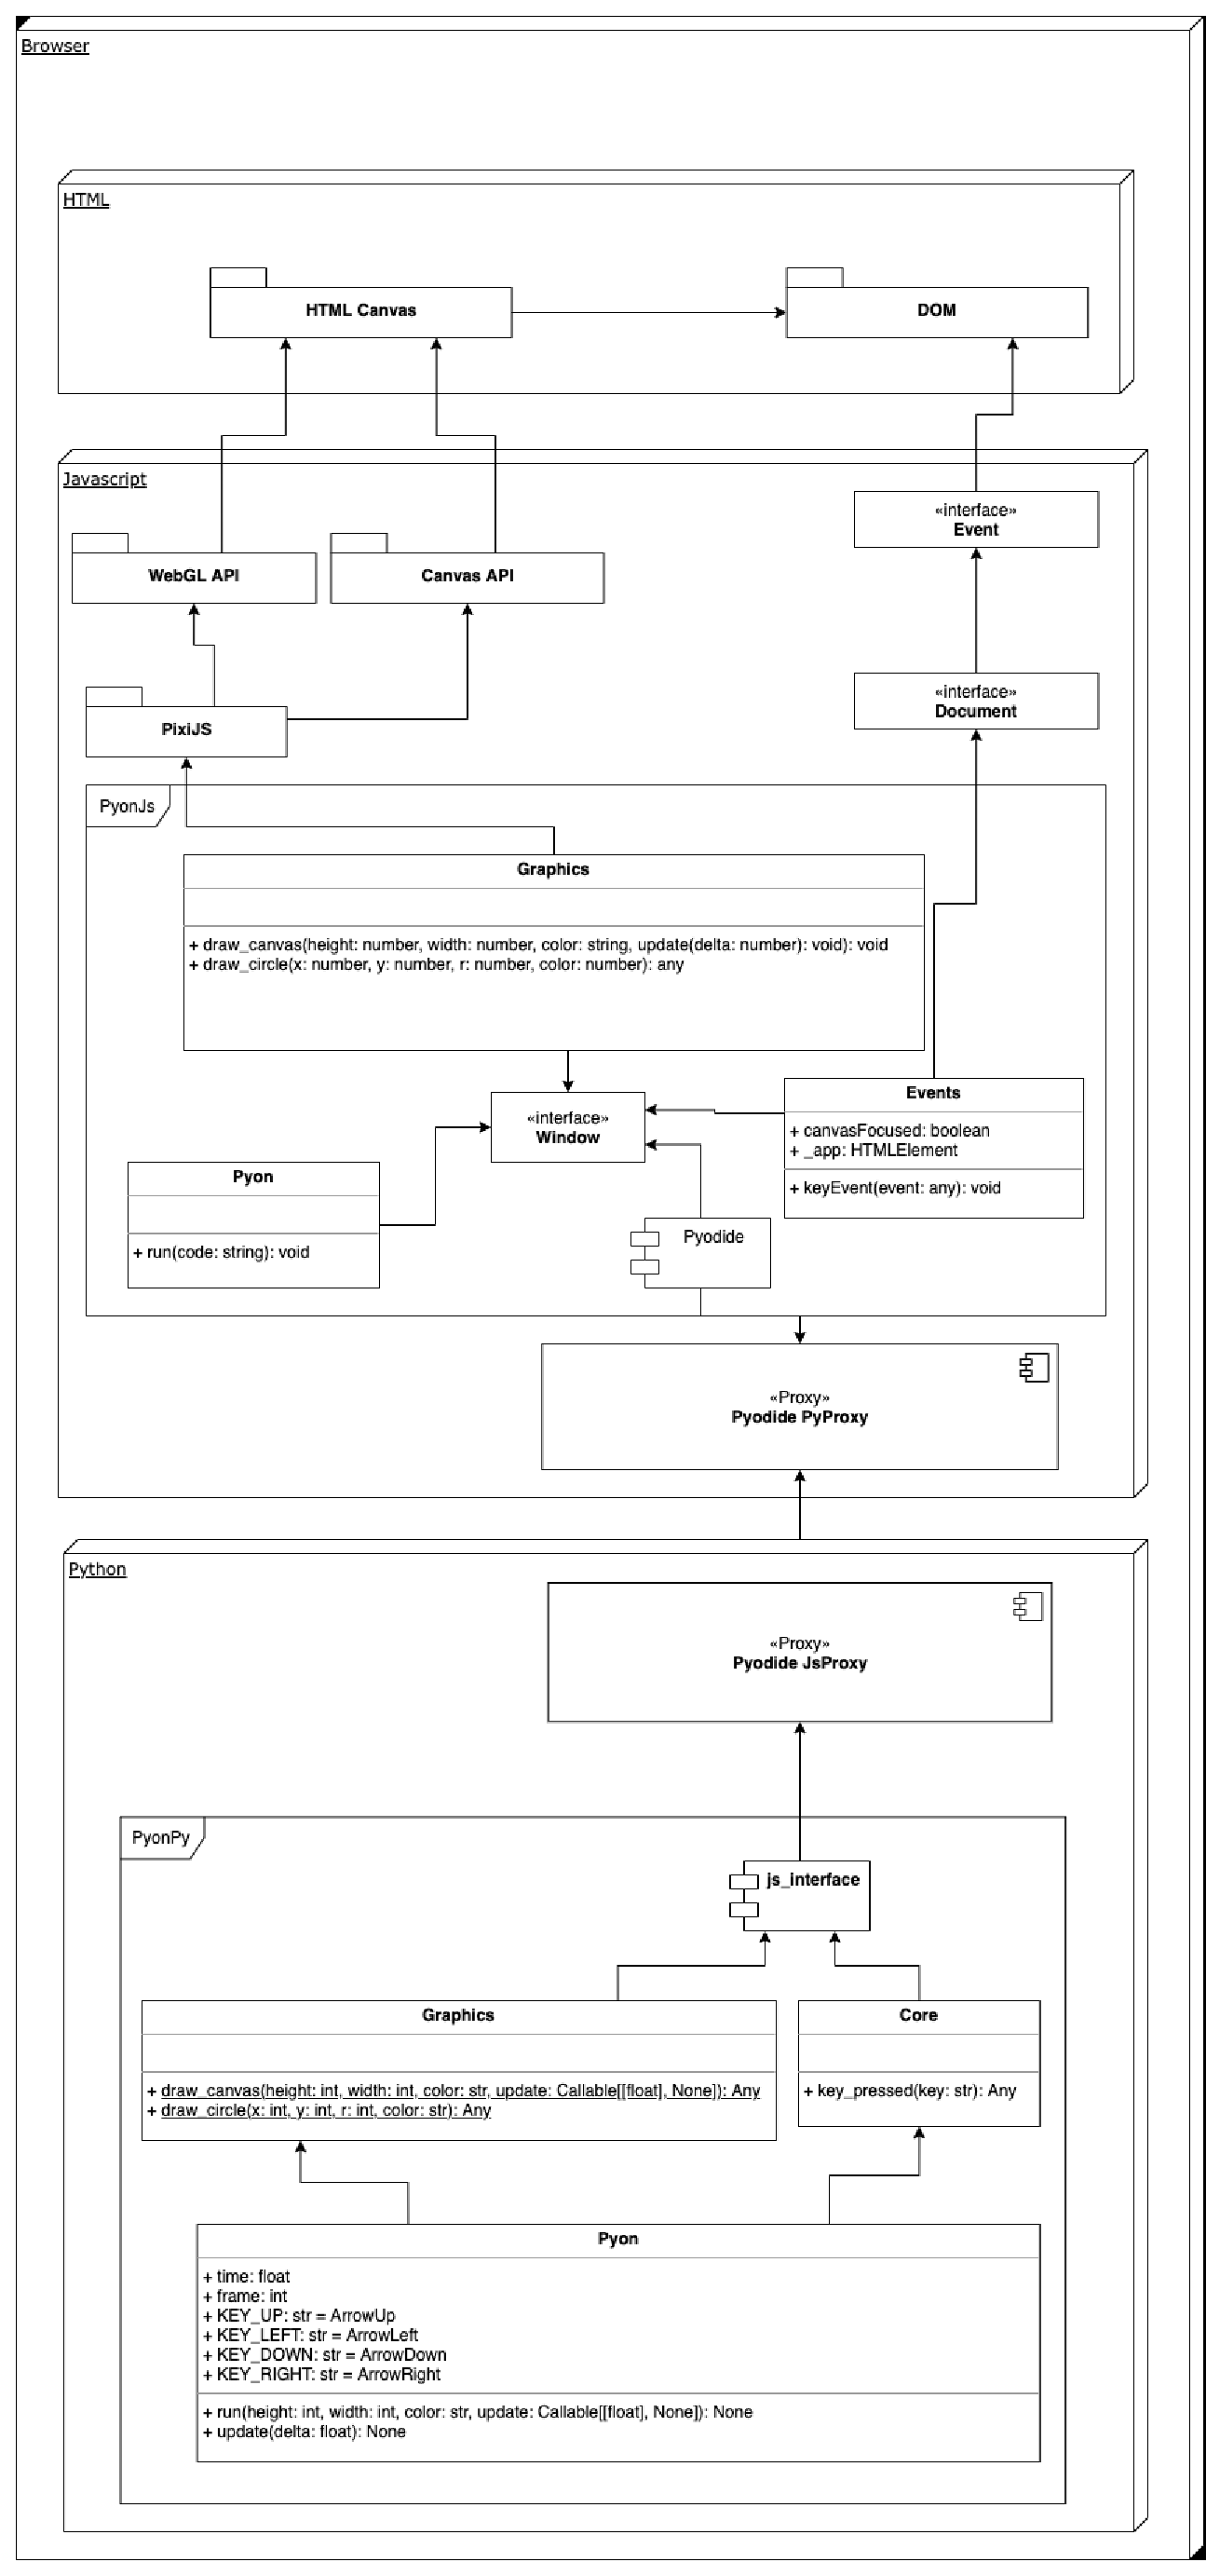
\includegraphics[trim={0 0 0 22cm},clip,keepaspectratio=true,scale=0.8]{figuras/Arquitetura.eps}
    \legend{Fonte: Autores}
    \label{fig:arquitetura}
\end{figure}

\section{Arquitetura}

\subsection{Camada Browser}

Representa a comunicação entre as sub-camadas HTML, JavaScript e Python. Com o python sendo interpretado para código C e compilado para Web Assembly pelo Pyodide.

\subsubsection{Camada HTML}

Representa a comunicação entre dois principais componentes HTML Canvas e DOM. 

\begin{itemize}
    \item \textbf{HTML Canvas:} responsável por possibilitar a rendenização de objetos 2D na DOM. 
    \item \textbf{DOM:} responsável por representar os objetos e captura de interações do usuário.
\end{itemize}

\subsection{Camada JavaScript}

\subsubsection{Pacote PyonJs}

Representa a comunicação da engine Pyon na camada JavaScript.

\begin{itemize}
    \item \textbf{Graphics:} Interface de comunicação entre a engine e o PixiJS, com suas funções disponibilizadas de forma global no Window.
    \item \textbf{Events:} Interface para monitoramento dos eventos de interação com a DOM, sendo o estado de cada evento atualizado de forma global no Window.
    \item \textbf{Pyon:} Interface da engine onde seu propósito é compilar o código criado pelo aluno através da instância disponívei no Window do Pyodide.
\end{itemize}

\subsection{Camada Python}

\subsubsection{Pacote PyonPy}

Representa a comunicação da engine Pyon na camada Python. Todo o código do usuário vai interagir com esta camada, e não com o JavaScript. 

\begin{itemize}
    \item \textbf{Graphics:} Interface de comunicação entre a engine e o Graphics da camada de JavaScript.
    \item \textbf{Core:} Interface para monitoramento dos eventos de interação entre a engine e o Events da camada JavaScript.
    \item \textbf{Pyon:} Interface que implementa atributos e funcionalidades que estarão disponíveis durante a execução do código recebido pelo PyonJS da camada JavaScript.
\end{itemize}
